%\chapter{General}
\thispagestyle{empty}

\begin{center}


\textbf{\LARGE{PILOT'S OPERATING HANDBOOK 
\\[0.5in]
}
}
\end{center}

\begin{figure}[h]
\centering

\includegraphics[width=1\textwidth]{vans-aircraft-logo.eps}
\label{fig:logo}
\end{figure}

\begin{center}

\textbf{\Huge{RV7 - 200HP C/S}}\\[0.5in]
\end{center}

\begin{figure}[H]
\centering
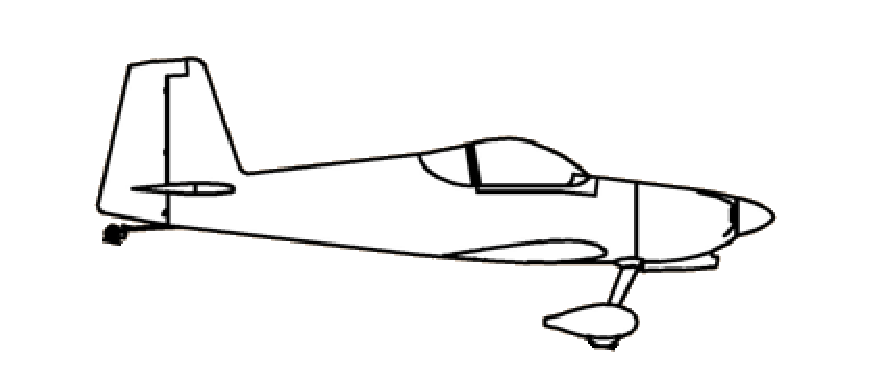
\includegraphics[height=0.15\textheight]{cover_rv.eps}
\end{figure}

\begin{center}
\begin{tabular}{ l r }
Serial No. & \textit{71334} \\ 
Registration No. & \textit{ZU-WAB} \\[0.25in]
\end{tabular}
\end{center}


\begin{center}
%THIS HANDBOOK INCLUDES THE MATERIAL REQUIRED TO BE FURNISHED TO THE PILOT BY THE REGULATIONS AND ADDITIONAL INFORMATION PROVIDED BY THE MANUFACTURER AND CONSTITUTES THE APPROVED AIRPLANE FLIGHT MANUAL.  \\[0.25in]

This Handbook follows GAMA Specification No. 1, \textit{Specification for Pilot's Operating Handbook}, issued February 15, 1975 and revised September 1, 1984.\\[0.25in]

First issue, \today
\end{center}








